\chapter{Literature Review}
\ifpdf
    \graphicspath{{Chapter1/Chapter1Figs/PNG/}{Chapter1/Chapter1Figs/PDF/}{Chapter1/Chapter1Figs/}}
\else
    \graphicspath{{Chapter1/Chapter1Figs/EPS/}{Chapter1/Chapter1Figs/}}
\fi


\section{Analysis of Complex Weighted Social Networks}

In this section the role of edge-weights in a social network is briefly surveyed. The drawback of using plain networks (without weights) is, it does not provide meaning in the real world sense. Therefore the analysis of these types of networks becomes very difficult. Hence it is necessary to assign weights to the ties between the nodes in a network. The weights are assigned to the edges by considering the features of the network and also identifying alternative definitions for the properties of graph theory. The benefits of this improvisation are:-
\begin{itemize}
\item Helps to find better methods for analysis
\item Obtain accurate results after analysis
\item Helps in better visualisation
\end{itemize}

The outcome of this process helps in predicting links and finding influential nodes in an efficient way.

Numerous networked structures can be found in different contexts such as technology, transportation infrastructure, social phenomenon and biological systems. These networks are very complex in nature and are heterogeneous in their capacity and intensity among connections. Before, These features were not considered for studies because links were represented either as present or absent. The two main example networks suitable for study are Scientific Collaboration network(SCN) and World-Wide Air transportation Network(WAN). These networks can be better analysed by assigning weights to the edges proportional to the intensity and capacity of the connections among the nodes. Appropriate metrics are defined to characterize the complex statistical properties and topological observations. The results provides a better insight into the structural hierarchies and descriptions.
The weights are assigned to the edges by considering both the properties of graph theory and the features of the network. The properties are centrality, betweenness, clustering coefficient and power-law behaviour. In some cases it is useful to come up with alternative definitions of centrality, cohesiveness and affinity. The conclusions show a more complete view of the complex networks. The importance of correlation between weights and topology of the networks is appreciated because it provides a better perspective of the network and these details cannot be obtained by the quantities just based on topological information. The study thus offers a quantitative and general approach to understand the complex architecture of real weighted networks.\cite{barrat2004architecture}

Feature weighting is an important application in content-based recommender systems. In content-based recommender systems, the main attributes are assigned weights. These weights are assigned based on their importance to users. A set of linear regression equations are used to estimate the weight values. These equations are obtained from social network graphs and are judged based on similarity of items.
In content based recommendation system, every item is represented as an attribute or a feature. These features hold numerical or nominal values. The similarity of two items is computed using various distance measures between features. The similarity values are then used to obtain a ranked list of recommended items. The edges are assigned different weights based on human judgement. A formula for computing similarity can be derived by using weights and function of attributes. The feature weights are estimated from social network graphs. A network is constructed using the results of existing recommender with items as nodes. The similarity among items can be induced using optimal feature weights. These optimal feature weights can be determined from linear regression equations. Thus feature weighting provides effective results from the recommender systems leading to rigorous analysis.\cite{debnath2008feature}

\noindent {\bf Role of edge weights} 

The structure of social networks influence the various dynamic processes of human interactions and communication. Weighted network models help to emulate the structure of real social networks They also help in displaying community structures with weak and strong internal links connecting the communities. The edge weights not only are important for dynamic processes but also in the formation of network structure itself. Weighted social networks can be designed to yield proper weight-topology correlations. They help to generate opinion formation models. Link weights not only make the model more realistic for describing human interactions in a social network but also generate a clear community structure. Thus it can be concluded that interaction weights play an important role in social dynamics. \cite{toivonen2007role}

\noindent {\bf Method : Attribute weight assignment}

This component mainly aims to assign a weight to each attribute in a network. It allows to represent attribute importance within a defined context. The assignment of weights depends on the framework created for the network structure. It can be assigned manually or computed automatically. Manual assignment allows users to include their preferences and inputs. Automatic assignment is provide to allow considering the social network characteristics. However, both can be used. The weight assignment to attributes is based on Inverse Functional Property(IFP). An algorithm can be designed for the process of assigning weights to attributes. The important steps of the algorithm are:

\begin{itemize}
\item Computing the importance of each attribute by crawling the related social networks.
\item Convert the input data into useful representation.
\item Computing the similarity score between each pair of similar attributes.
\item Data analysis step
\item Associating each attribute with a set of similarity scores in order to compute the final weight.
\end{itemize}

Data aggregation/fusion techniques are needed to combine information from different sources and obtain one result for a more accurate decision. These techniques several approaches such as probabilistic models, evidence theories and classical functions. An important application of attribute weight assignment is profile matching in social networks.  It also helps in better understanding of inter-social network operations and functionalities. \cite{raad2010user}

\noindent {\bf Example:}
A scientific collaboration network is considered for analysis. The strength of collaborative ties are estimated. A formula for assigning weights to the edges is devised by making suitable assumptions. Social network analysis algorithms are applied on the weighted network and the results are examined. The improvements in the performance of SNA algorithms on weighted networks are observed and reasons for the same are stated. \cite{clauset2009power}

\section{Influence Analysis}\label{SecIA}

An attempt is made using social network analysis to answer the question ''Who are the most influential individuals in a network?''. Influential individuals are said to be those who are capable of convincing other individuals to adapt their attitude, behaviour, or belief to that of the former. Identifying the key influential individuals in a network can play a key role in the introduction, longevity, and fidelity of program implementation.
 
Given a set of weighted, directed relations among the individuals in a large network, clustering  based on the fast greedy algorithm \cite{clauset2004finding} is initially performed on this network to identify closely related sub-networks of individuals. Next, these clusters are analysed one by one as independent organizations. The PageRank \cite{brin1998anatomy} of all the individuals in the cluster are computed in order to determine their local standing (relative to  the cluster). For each individual A, the weights that A has assigned to every other individual in the cluster is multiplied by the PageRank of A in order to incorporate the influence of A. With these updated weights, the in-degree centrality (also known as in-ties) is computed and then used as a measure of the total communication directed at each individual. For each individual, the in-tie measure indicates how well other individuals in the cluster weigh this individual. Individuals who receive higher scores are considered more influential in the network.

In order to visualize the distribution of the in-degree measure within an organization, the in-degree scores for all individuals can be sorted in descending order and then graphed, resulting in a ''scree'' plot. This technique allows a researcher to get a sense of the distribution of in-ties for all the actors in the organization. Now the focus is on establishing a defensible threshold for identifying the most influential individuals in an organization. Visual inspection of the scree plot can make identifying influential’s an onerous task. As an alternative, four reproducible methods are investigated for categorizing influential individuals in an organization. A detailed explanation of these methods follows. These explanations and further details can be found in \cite{cole2009identifying}.

\noindent {\bf Method 1 - Absolute Cut Score}

The simplest and most intuitive method for determining a cut score is to set a predetermined absolute value above which individuals are deemed influential and below which they are not. Graphically, this can be accomplished by superimposing a horizontal line over the in-degree scree plot. Those individuals whose influence scores are above the horizontal line are then categorized as influentials. However, since this method is based entirely on a single point and is determined independent of variation in the distribution of in-ties, it can result in the situation where every individual (or no individual) in a network can potentially be deemed influential since the criterion is absolute, not relative.

\noindent {\bf Method 2 - Fixed Percentage of Population}

An alternative method of identifying influentials is to select a fixed percentage of the population as influential. If the top 20\% of individuals in an organization are to be categorized as influentials, this is equivalent to selecting the leftmost 20\% of the individuals in the graph. Those individuals to the left of a vertical line superimposed over the scree plot are categorised as influential. As with the Absolute Cut Score, this method identifies individuals as influential independent of the variation of in-ties. It ensures that a given percentage of individuals in the organization are identified as influential and their identification is based upon their performance relative to the performance of other individuals in the organization.

\noindent {\bf Method 3 - Standard Deviation}

Unlike the first two approaches, the Standard Deviation method focuses on the variation in the distribution of ties. This procedure requires calculation of the mean and standard deviation of the number of in-ties. Then we create a horizontal line two standard deviations above the mean, which can be superimposed over the scree plot. This horizontal line approach is similar to the Absolute Cut Score (Method 1), however, the Standard Deviation method does not choose a cut score a priori, instead it utilizes the observed data in determining where to set the cut point. Under this method, those individuals whose in-degree scores are above this line are marked ''influential.''

\noindent {\bf Method 4 - Random Permutation}

Through the use of random permutations, Method 4 produces results which identify those individuals who received significantly more in-ties than would have occurred by chance alone. This method capitalizes on the creation of a sampling distribution of potential networks that could have occurred, conditional on the fixed row marginal’s or (out-tie distribution). In order to obtain a sampling distribution of influence for the network, the graph (nodes and edges) is modeled as an exponential random graph \cite{hunter2008ergm}. Then the edges are randomly reassigned to individuals in the network keeping the out-degree distribution fixed. By performing one thousand such random permutations the sampling distribution of influence (that is, in-degree distribution) is derived under conditional independence.
 
The ties are not completely independent, as we restrict their new random locations to only emanate from their original sources in the actual data (i.e. the row marginals are fixed). However, in forcing this restriction, we are able to create a sampling distribution of influence that is comparable to our actual data. The result is the distribution that would arise by random chance, given the set of survey responses, and therefore can be used to identify those individuals whose influence is statistically greater than random chance. Once this is completed, individual influence scores are recalculated according to the in-degree measure described earlier. If an individual’s actual influence score is higher than his/her ranked counterpart for 95\% of the random iterations, then the individual is labeled a “significant influential” at the $p < .05$ level.

\noindent {\bf Sampling Based Clustering}

It is abundantly clear that performing influence analysis following clustering of an entire
network of enormous size becomes computationally infeasible once a threshold size is breached.
This implies that somehow or other identification of the subnetworks lying inside the
huge network is essential. A new technique is proposed here which can identify the important
subnetworks without exploring the entire network. Random sampling techniques are employed
in this technique. \cite{ross2014introduction}

\section{Link Prediction}\label{SecLP}

Social networks are structures whose nodes represent people or other entities embedded in a social context, and whose edges represent interaction, collaboration, or influence between entities. These networks grow quickly over time with the additions of new entities and interactions between them. The main goal here is to understand how they evolve over time. Link Prediction studies and defines models that help in understanding the underlying evolution.

Link Prediction addresses the problem of predicting links that are either missing or may appear in the future \cite{liben2007link}. There are many factors that can be considered while predicting links between entities of a network that do not exist currently. These factors may be external or internal to the network. For example, two authors in a collaboration network who do not know each other and do not have any short chain of acquaintances may start collaborating in the near future, if one of the authors move to a different university geographically located where the other author works. In this case, the chances of them collaborating increases. These factors are external to the network. Predicting links using external factors such as these is a difficult task. However, there are factors that are internal to the network using which predicting links become much easier. These methods use network topology to predict links. 

Link prediction has applications in various fields like in large organizations where predicting promising links between its employees helps in the development of the organization. In monitoring terrorist networks where links between individuals can be predicted even though no interactions are observed between them. It also finds applications in monitoring and controlling computer viruses that use email as a vector. It can be used to provide recommender systems, to predict unobserved links between protein-protein interaction networks in biological system.

\noindent {\bf Problem Description:}

Consider a graph $G (V, E)$ where $V$ is the set of nodes and $E$ is the set of links in the graph $G$. Multiple links and self connections are not allowed in $G$. Let $U$ represent the universal set consisting of all possible links. Then, the set of non-existent links is $U-E$. The task of link prediction is to predict the missing links or links that may occur in future in the set $U-E$. 

\noindent {\bf Metrics:}

In order to check the accuracy of links predicted, the observed links $E$ is divided two parts: The training set, $E_T$ and the probe set, $E_P$. The training set is used as known information while the probe set is used for testing. No information of the probe set is used for prediction purposes. 

There are two standard metrics used to test the accuracy of the prediction algorithms: Area Under the receiver operating characteristic Curve (AUC) and Precision. Every prediction algorithm assigns score to links in $U-E_T$ depicting the likelihood of its existence. These scores are arranged in decreasing order such that given a particular link; its occurrence is more likely than the link below it in the ordered list. The AUC evaluates the algorithms performance based on the overall list while Precision focuses on only L links with top scores.
	
\noindent {\bf i) AUC:}

The AUC value gives the probability that a random chosen missing link (a link in $E_P$) is given higher score than a randomly chosen non-existent link (a link in $U-E$). During algorithmic implementation, we randomly select a non existing link from $U-E$ and a missing link from $E_P$ to compare their scores \cite{lu2011}. 

If all scores are generated from identical distribution then the value of AUC will be 0.5. Thus, the degree to which the value exceeds 0.5 indicates how better the algorithm performs compared to pure chance. 

\pagebreak
\noindent {\bf ii) Precision:}

The Precision value is defined as the ratio of relevant items selected to the number of items selected \cite{lu2011}. Clearly, higher the precision value higher the prediction accuracy.

\noindent {\bf Methods:}

\noindent {\bf Similarity Based Algorithms:}

The simplest of all prediction algorithms is the similarity based algorithms where every pair of nodes $x$ and $y$, are assigned a score $S_{xy}$ which directly defines their similarity. All non-observed links are ordered according to their similarity score and links connecting similar nodes are expected to have higher existence likelihoods. 

Similarity between the nodes can be defined using the attributes of the nodes i.e., two nodes are more similar if they have many common features. However attributes of nodes are generally hidden and thus to define the similarity of nodes we concentrate on the structural similarity between the nodes which depends on the network structure.

Similarity based methods can be classified in a number of ways be it, local vs global, parameter-free vs parameter-dependent or node based or path based. They can also be classified as structural equivalence where the assumption is that the link indicates similarity between its end points, and regular equivalence where the assumption is that two nodes are similar if their neighbours are similar.

\noindent {\bf Local similarity indices:}

These indices consider only information related to the immediate neighbourhood of the nodes. Some of the well known local indices are

\noindent {\bf i) Common Neighbours (CN):}

The common neighbor algorithm is one of the simplest and most commonly used algorithms for predicting links in a network. The concept of common neighbor was applied by Newman in reference to collaboration graph to verify correlation between common neighbors of two nodes say $u$ and $v$ of a network $G$ and to compute the probability that they will collaborate in the near future \cite{newman2001clustering}. 

\noindent {\bf ii) Jaccard’s Index:}

The Jaccard’s coefficient algorithm is one of the most commonly used algorithms in computing similarity coefficient during information retrieval. It is also referred to as Jaccard’s index of similarity \cite{jaccard1901etude}.  It was primarily used as a similarity computing algorithm in the works of Salton and McGill on information retrieval.

\noindent {\bf iii) Adamic Adar (AA) :}

The Adamic Adar (AA) algorithm is based on the well established results in sociology that friends tend to be similar \citep{carley1991theory, feld1981focused}. Given any two people or users in our case, more things they have in common, more likely they are to become friends; more likely links are created between them in the near future. Similarity is measured by analysing the links of each user. While trying to evaluate whether a particular user can be linked to another user, we sum the number of items both the users have in common. Items that are unique to few people are weighted more while items that are common among many people are weighted less. The Adamic Adar Index \cite{adamic2003friends} was proposed by L.A. Adamic and E.Adar. It assigns more weight to less connected members. 

Experimental results on different social networks show that these methods are time consuming and are not feasible for large social networks. It uses different network information such as structural properties of the network, node attributes to determine the link existence between a pair of nodes i.e., it concentrates only on the existence of the links and not the properties of individuals that the nodes represent. However, it does not use other information such as behaviour of nodes. In order to overcome such drawbacks, hybrid methods are developed which considers local information as well as community information.

Hybrid methods using community information consider that there is high concentration of existence of links within communities and low concentration between the communities. Given a network, we compute the probabilities of link existence and non existence of all the links in the network. To determine the probability of a non existent link, we establish a hybrid method which uses Bayesian theory.

For an undirected network, according to Bayesian theory \cite{hastie2005elements}, the posterior probabilities of the link existence and nonexistence between a pair of nodes $(x,y)$, given its set of all common neighbors can be defined \cite{valverde2014link}. 

We define the set of all common neighbours as sum of common neighbours within common groups and common neighbours outside of common groups. In order to determine the probability of common neighbours given the existence of links between $x$ and $y$, we have to consider the number of common neighbours within common groups by number of all common neighbours. Similarly, in order to determine the probability of common neighbours given the non-existence of links between $x$ and $y$, we have to consider the number of common neighbours outside of common groups by number of all common neighbours.

In order to determine the link likelihood between $x$ and $y$, we define the similarity
score as the ratio of probability of link existence between $x$ and $y$ to probability of link non existence \cite{valverde2014link}. 
On simplification we get the similarity score for Within and Outside of Common Groups (WOCG) \cite{valverde2014link} as follows :
$$s_{x,y}^{WOCG} = \frac{|\Lambda_{x,y}^{WCG}|}{|\Lambda_{x,y}^{OCG}|}\times \Omega,$$
where $\Omega$ is a constant.


\section{Time Series Analysis}\label{SecTSA}

Time series analysis is an approach where  data or datasets are analysed over discrete intervals of time such that processed data for a period of time say $t_0$ serves as an input to time slot $t_1$. The efforts here are to use novel methods so as to analyze the network, establish relations among nodes, predict and forecast the behavior of social networks over a given period of time. With the help of temporal analysis methods and the underlying algorithms supporting them temporal distances and metrics are determined. \citep{santoro2011time,o2010tweets}

Time series analysis consists of various steps namely estimation, prediction, query processing, result analysis and stimulation in order to get precise and aesthetically better results. It is used in engineering, business activities and sees application in various fields. Here, the attempt is to try and explore how a given social network reacts over time and how it behaves with the addition of new users, or which users tend to interact among each other, estimation of likelihood that a person X may collaborate with another person Y in future. 
\citep{o2010tweets,tang2009temporal}


\section{Power Law}
A Power Law is a mathematical relationship between two quantities, where one quantity varies as a fixed power of another.
A network whose degree distribution follows a power law is called a scale-free network. A graph for power law follows
a long/heavy tailed distribution. The power law graph can be used to demonstrate the ranking of popularity of nodes
and predict the region of interest of a particular node in a network. The procedure for verifying power law for a
network is a dynamic approach, where data are analysed over a period of time.
Power law distributions are very much widespread in computer science. They are also often referred to as heavy-tail distributions,
Pareto's distribution, Zipfian distributions etc.

The important discoveries made by Mitzenmacher are:-
The most important one is that much of what we in the computer science community have begun to understand and utilize about power law and lognormal distributions has already been known in other sciences such as economics and biology. Very similar models to the dynamically growing webgraph model which results in a power law distribution have been used way back in 1920's.
A second discovery is the argument over whether a lognormal or power law or any other distribution is a better fit for some experimentally observed distribution has been repeated across many fields like chemistry, ecology, information theory over many years since 1950's.
Another discovery is that the distributions like power law, lognormal are necessarily connected. A basic model upon variations may follow any distributions. \cite{mitzenmacher2004brief}
Many experimental quantities have tendency towards a typical value. Ex: Speeds of cars on highways, weights of a fruits in a store. All these things vary but the distributions make the typical value representative of most important observations. There are many such distributions but the power law is known for its mathematical properties which leads to surprising consequences and for its appearance in different natural and man-made phenomena. The population of cities, intensities of earthquakes follow power law distribution. \cite{clauset2009power}
The recent observations suggest that the power law is also used to study the topology of internet. From this study, new and efficient protocols can be designed that take advantage of its topological properties. A more accurate artificial models can be created for simulation purposes and also neighbours within a network can be predicted. This is helpful to analyze the geographical distribution of nodes. Power laws have been used to describe different characteristics of communication networks. Recent studies have observed that the preferential attachment and incremental growth are possible causes for power laws in some topologies. The World Wide Web also follows power law distribution. \cite{medina2000origin}
The latest trending application of power law distribution is in social networks. Most of the social networks follow power law distribution. Power law helps in predicting the relations among nodes and the region of interest for nodes in a network. For example, the power law is useful in predicting mutual friends or friends-of-friends in Facebook. It can also be used to demonstrate the ranking popularity of nodes in a social network. For example the increase in number of followers for a famous person in a social network can be predicted.
Example:
A common example to demonstrate the concept of power law is the city-population graph.
\begin{figure}
\centering
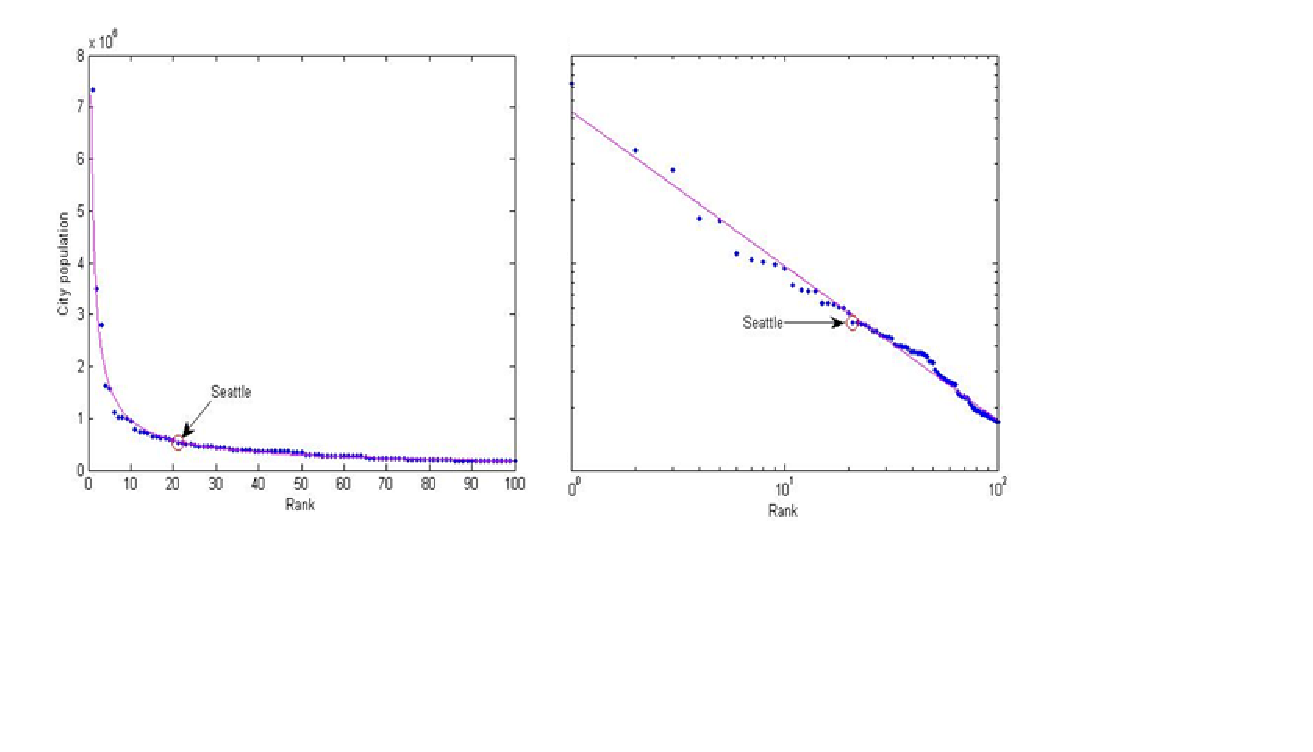
\includegraphics[scale=0.6]{Chapter1/PLgraph.eps}
\caption{City Population Graph}
\end{figure}

Important Observations:
\begin{enumerate}
\item The above graph follows power law distribution in its long-tail.
\item There are only few cities with very high population. There are more number of cities with less population
\item More people have moved from cities with low population to the cities with already high population
\item The rich-become-richer mechanism can be observed.
\end{enumerate}


% ------------------------------------------------------------------------


%%% Local Variables: 
%%% mode: latex
%%% TeX-master: "../thesis"
%%% End: 
